\documentclass{beamer}
%\usepackage{split}

\usepackage{amsmath}
\usepackage{amsfonts}
\usepackage{braket}
\usepackage{subcaption}
\usepackage{tikz}
\usepackage{xcolor}
\usepackage{svg}
\usetikzlibrary{positioning,shapes,arrows.meta}
%\usetikzlibrary{positioning,fit,backgrounds}
\usepackage{quantikz}
\usepackage[linesnumbered]{algorithm2e}
\usepackage{hyperref}
%\usepackage{hyperref,xcolor}
%\usepackage[ocgcolorlinks]{ocgx2}
\usepackage{cleveref}
\usepackage[backend=biber,style=alphabetic,sorting=ynt]{biblatex}
\addbibresource{./sample.bib}


\input{newcommands}


\newcommand*{\QACze}{ \mathbf{QAC}_{0} }
\newcommand*{\QNCzef}{ \mathbf{QNC}_{0,f} }
\newcommand*{\QNCze}{ \mathbf{QNC}_{0} }
\newcommand*{\QNCon}{ \mathbf{QNC}_{1} }
\newcommand*{\NCon}{ \mathbf{NC}_{1} }
\newcommand*{\noiseQNCon}{ noisy-$\QNCon$ }
\newcommand*{\QNC}{ \mathbf{QNC} }
\newcommand*{\QNCG}{ \mathbf{QNC_G} }
\newcommand*{\NC}{\mathbf{NC}}
\newcommand*{\QNCiG}{\mathbf{QNC_{G,i}}}



\usetikzlibrary{patterns, shapes.arrows}
\usepackage{tkz-graph}
\usetikzlibrary{decorations.pathmorphing}
\usepackage{tkz-berge}

\usetikzlibrary{intersections}

\usepackage{cancel}
\begin{document} 

%\newcommand*{\Tr}{\textbf{Tr }}


\begin{frame}
  \title{Local Decoder.}
    \author{David Ponarovsky}
    \date{\today}
    \titlepage
\end{frame}


\begin{frame}

\frametitle{Introduction}
\begin{block}{Today:}
\begin{itemize}
  \item Proof. 
    \begin{enumerate}
      \item Local Decoders.
   %   \item A 
  %    \item B
    \end{enumerate}
%  \item New experimental results.  
 % \item Answering the code teleportation.  
\end{itemize}
\end{block}
\end{frame}

% ------------------------------------------------ $ 
  
\begin{frame}
  \frametitle{Our Code}

  \begin{block}{Code}
    In this session, we consider LDPC codes, where each bit adjoins to $\Delta_{1}$ checks, and each check adjoins to $\Delta_{2}$ bits. We denote by $\Delta = \Delta_{1}\Delta_{2}$.
  \end{block}


\end{frame}

\begin{frame}
  \frametitle{Local Decoder} 
  
  \begin{block}{definition}
    We say that $D$ is a local decoder if when applied against $2p(1-p)$-depolarized channel: 
    \begin{itemize}
      \item  There exists function $M : (0,1) \rightarrow (0,1) $ such that the probability of each bit being flipped is $M(2p(1-p)) < p^{\frac{100}{99}}$.
      \item There is a constant $l$ such that for any bit, there are only $(\Delta)^{l}$ bits on which the event of it being flipped depends.
    \end{itemize}
For example, if we take $k$ large enough and consider the $(n,k)$-Toric, then both the swift-rule and the flip upon majority are local decoders.
  \end{block}
\end{frame}


\begin{frame}

    \begin{figure}[H]
  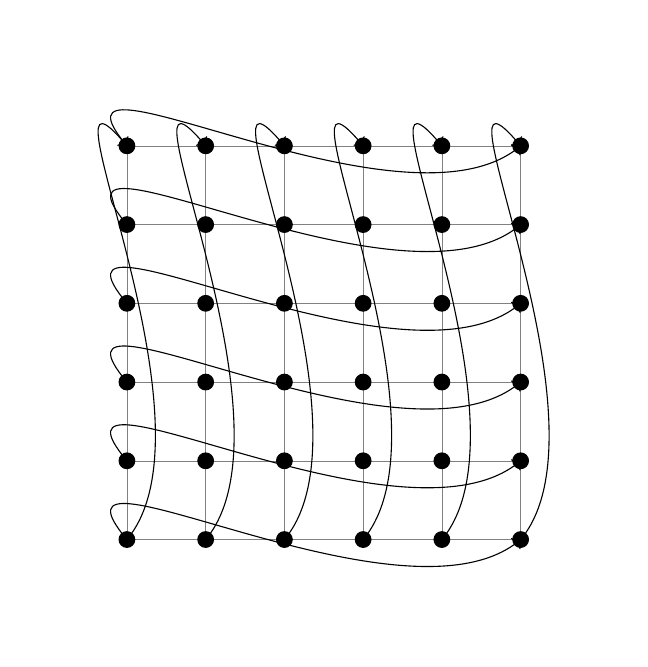
\begin{tikzpicture}
  \draw[step=1cm,gray,very thin] (0,0) grid (5,5);
  \foreach \x in {0,1,2,3,4,5}
  \foreach \y in {0,1,2,3,4,5}
  {
  \node[draw,circle,inner sep=2pt,fill] at (\x,\y) {};
}
\draw[ -> ]  (0,0) to [out=50, in=130] (0,5);
\draw[ -> ]  (1,0) to [out=50, in=130] (1,5);
\draw[ -> ]  (2,0) to [out=50, in=130] (2,5);
\draw[ -> ]  (3,0) to [out=50, in=130] (3,5);
\draw[ -> ]  (4,0) to [out=50, in=130] (4,5);
\draw[ -> ]  (5,0) to [out=50, in=130] (5,5);
\draw[ -> ]  (0,5) to [out=130, in=220] (5,5);
\draw[ -> ]  (0,4) to [out=130, in=220] (5,4);
\draw[ -> ]  (0,3) to [out=130, in=220] (5,3);
\draw[ -> ]  (0,2) to [out=130, in=220] (5,2);
\draw[ -> ]  (0,1) to [out=130, in=220] (5,1);
\draw[ -> ]  (0,0) to [out=130, in=220] (5,0);

\end{tikzpicture}
\caption{On the left is the Toric Graph. On the right are cross and face checks.}
\label{fig:Toric}
\end{figure}



\end{frame}


\begin{frame}

    \begin{figure}[H]
  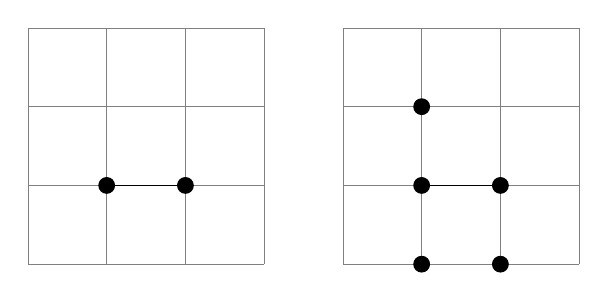
\begin{tikzpicture}
  \draw[step=1cm,gray,very thin] (0,0) grid (3,3);
  \draw[step=1cm,gray,very thin] (4,0) grid (7,3);
  \draw  (1,1) -- (2,1);
  \draw  (5,1) -- (6,1);
  \node[draw,circle,inner sep=2pt,fill] at (1,1) {};
  \node[draw,circle,inner sep=2pt,fill] at (2,1) {};
  \node[draw,circle,inner sep=2pt,fill] at (5,1) {};
  \node[draw,circle,inner sep=2pt,fill] at (6,1) {};
  \node[draw,circle,inner sep=2pt,fill] at (5,0) {};
  \node[draw,circle,inner sep=2pt,fill] at (5,2) {};
  \node[draw,circle,inner sep=2pt,fill] at (6,0) {};
\end{tikzpicture}
\caption{On the left is the Toric Graph. On the right are cross and face checks.}
\label{fig:Toric}
\end{figure}

\end{frame}


\begin{frame}
  
If both checks are unsatisfied, then flip the bit. Denote by $\kappa$ the number of edges adjacent to those checks. Then the probability of failure is less than:
  \begin{equation*}
    \begin{split}
      &(1-p)2^{\kappa - 1} \cdot p^{2} + p 2^{\kappa-1} p \le p^{2} 2^{\kappa} \\
      & \le p^{\frac{100}{99}}
    \end{split}
  \end{equation*}
  For $p$ small enough. 


  \inb{ Also correct for the local stochastic noise model. $\le Cp^{2}2^{\kappa}$. }
\end{frame}



\begin{frame}

    \begin{figure}[H]
  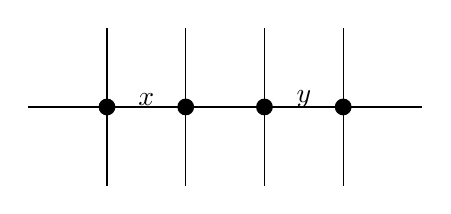
\begin{tikzpicture}
  \node[draw,circle,inner sep=2pt,fill] at (1,1) {};
  \node[draw,circle,inner sep=2pt,fill] at (2,1) {};
  \node[draw,circle,inner sep=2pt,fill] at (3,1) {};
  \node[draw,circle,inner sep=2pt,fill] at (4,1) {};
  \draw  (0,1) -- (1,1);
  \draw  (1,1) -- (2,1);
  \draw  (2,1) -- (3,1);
  \draw  (3,1) -- (4,1);
  \draw  (4,1) -- (5,1);
  \draw (1,0) -- (1,1) -- (1,2);
  \draw (2,0) -- (2,1) -- (2,2);
  \draw (3,0) -- (3,1) -- (3,2);
  \draw (4,0) -- (4,1) -- (4,2);
  \node at (1.5,1.1) { $x$ };
  \node at (3.5,1.1) { $y$ };
\end{tikzpicture}
\caption{On the left is the Toric Graph. On the right are cross and face checks.}
\label{fig:Toric}
\end{figure}

\end{frame}

\begin{frame}
  Denote by $\kappa^{\prime}$ the number of bits adjacent to a check that is adjacent to $x$ but not to $y$ ($\kappa^{\prime} = \kappa -1$). The probability that $D$ fails to 'correct' both $x$ and $y$, conditioned on no (q)bit in the intersection of their light cone being flipped, is less than:

\begin{equation*}
  \begin{split}
    &(1-p)^{2} \left(2^{\kappa^{\prime}-1}p^{2}\right)^{2} + 2(1-p)p \left( 2^{\kappa^{\prime}-1} p \cdot 2^{\kappa^{\prime}-1} p^{2}  \right) \\
    & + p^{2}\left( 2^{\kappa^{\prime}-1} p \right)^{2} \\ 
    \le & \left( (1-p)2^{\kappa - 1} \cdot p^{2} + p 2^{\kappa-1} p \le p^{2} 2^{\kappa} \right)^{2} \\
    \le & \left( p^{\frac{100}{99}} \right)^{2}
  \end{split}
\end{equation*}
  \inb{ In the local stochastic noise model the $C$ is outside the power namely. $\le C \left( p^{\frac{100}{99}} \right)^{2}$ }
\end{frame}



\begin{frame}

    \begin{figure}[H]
  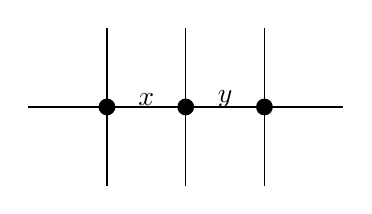
\begin{tikzpicture}
  \node[draw,circle,inner sep=2pt,fill] at (1,1) {};
  \node[draw,circle,inner sep=2pt,fill] at (2,1) {};
  \node[draw,circle,inner sep=2pt,fill] at (3,1) {};
  \draw  (0,1) -- (1,1);
  \draw  (1,1) -- (2,1);
  \draw  (2,1) -- (3,1);
  \draw  (3,1) -- (4,1);
  \draw (1,0) -- (1,1) -- (1,2);
  \draw (2,0) -- (2,1) -- (2,2);
  \draw (3,0) -- (3,1) -- (3,2);
  \node at (1.5,1.1) { $x$ };
  \node at (2.5,1.1) { $y$ };
\end{tikzpicture}
\caption{On the left is the Toric Graph. On the right are cross and face checks.}
\label{fig:Toric}
\end{figure}

\end{frame}


\begin{frame}
In the above case, where $y$ is in the light cone of $x$ and vice versa, the condition that there is no faulty bit on their light cone restricts to the case that both $x$ and $y$ weren't flipped, and no edge adjacent to the middle vertex is flipped. Thus, each of them sees at most one unsatisfied check. Thus, $D$ doesn't flip them. Namely, the probability that $D$ fails is zero $\le p^{\frac{100}{99}}$.
  \inb{ Also correct for the local stochastic noise model. }
\end{frame}



\begin{frame}


  \begin{figure}[h]
    \centering
    \includegraphics[width=0.8\textwidth]{2d-color-code.png}
    \caption{2d color code}
    \label{fig:2dcolorcode}
  \end{figure}

\end{frame}



\begin{frame}

    \begin{figure}[H]
  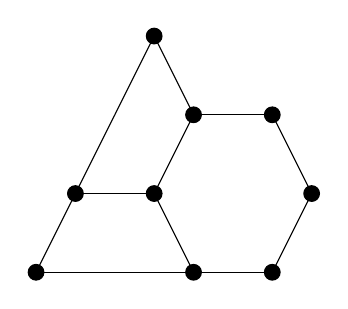
\begin{tikzpicture}
  \node[draw,circle,inner sep=2pt,fill] at (0,0) {};
  \node[draw,circle,inner sep=2pt,fill] at (2,0) {};
  \node[draw,circle,inner sep=2pt,fill] at (3,0) {};
  \node[draw,circle,inner sep=2pt,fill] at (0.5,1) {};
  \node[draw,circle,inner sep=2pt,fill] at (1.5,1) {};
  \node[draw,circle,inner sep=2pt,fill] at (3.5,1) {};
  \node[draw,circle,inner sep=2pt,fill] at (3,2) {};
  \node[draw,circle,inner sep=2pt,fill] at (2,2) {};
  \node[draw,circle,inner sep=2pt,fill] at (1.5,3) {};
  \draw  (0,0) -- (0.5,1);
  \draw  (0.5,1) -- (1,2);
  \draw  (1,2) -- (1.5,3);
  \draw  (0,0) -- (2,0);
  \draw  (2,0) -- (3,0);
  \draw  (3,0) -- (3.5,1);
  \draw  (3.5,1) -- (3,2);
  \draw  (3,2) -- (2,2);
  \draw  (2,2) -- (1.5,3);
  \draw  (2,2) -- (1.5,1);
  \draw  (1.5,1) -- (0.5,1);
  \draw  (1.5,1) -- (2,0);
\end{tikzpicture}
\caption{On the left is the Toric Graph. On the right are cross and face checks.}
\label{fig:Toric}
\end{figure}



\end{frame}



\begin{frame}


  \begin{figure}[h]
    \centering
    \includegraphics[width=0.8\textwidth]{3d-color-codes-1.png}
    \caption{3d color code}
    \label{fig:3dcolorcode}
  \end{figure}

\end{frame}



\end{document}
